\KMMTitlePage


\section{Palanki mokymuisi aplinka}


\begin{frame}{Protokolas}{\secname}
\begin{ApBox}
\onslide<2->{\textbf{Protokolas}}
\onslide<3->{— tai susitarimas ar taisyklių rinkinys, kaip reikia elgtis tam tikroje situacijoje.}
\end{ApBox}
\end{frame}


\begin{frame}
\centering

\includegraphics[scale=0.25]{kmm_logo_sneeze.jpg}
\end{frame}


\begin{frame}
\centering

\includegraphics[scale=0.25]{kmm_logo_hand.jpg}
\end{frame}


\begin{frame}
\centering

\includegraphics[scale=0.25]{kmm_logo_elbow.jpg}
\end{frame}


\begin{frame}
\centering
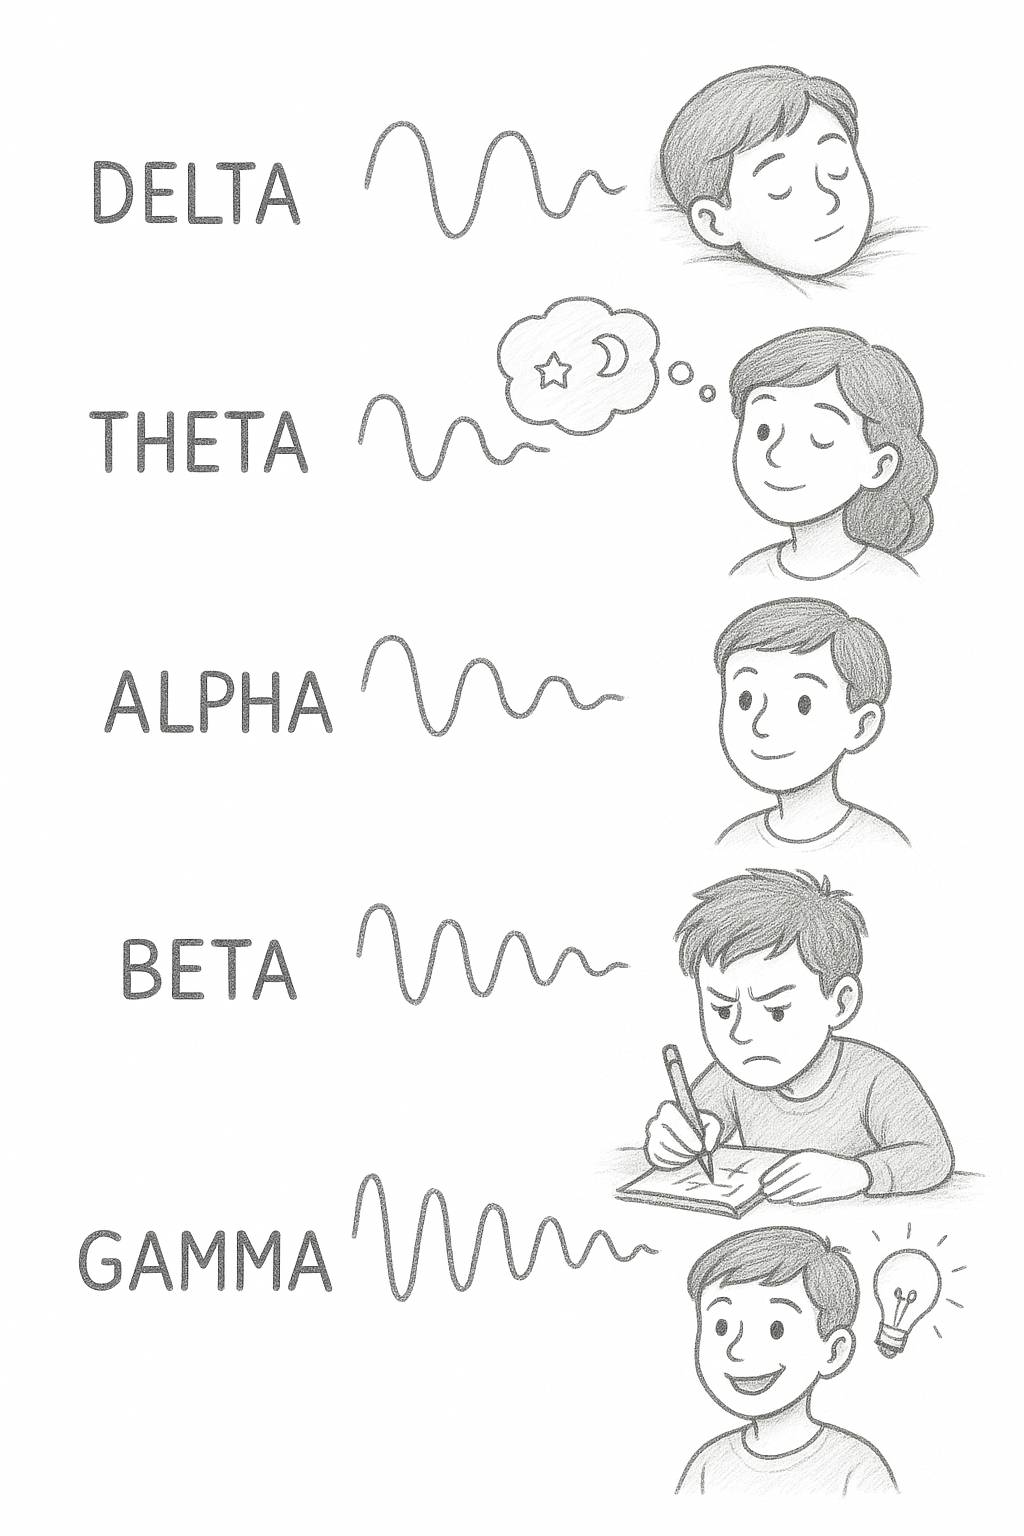
\includegraphics[scale=0.16]{brainwaives_illustration.jpg}
\end{frame}


\section{Mokyklos protokolai}


\section{Matematikos klasės protokolai}


\section{Reikalingos mokymosi priemonės}


\begin{frame}{Reikalingos mokymosi priemonės}{\secname}
\begin{itemize}[label=\textbullet]
\item<2-> Sąsiuvinis langeliais storas klasės darbams (rekomenduoju A4 formato be metalinio žiedinio sujungtuvo).
\item<3-> Sąsiuvinis langeliais namų darbams (pageidautina, kad būtų plonas ir galite nusipirkti jau daugiau nei vieną).
\item<4-> Keletas rašiklių (kad turėti, jei ką draugui paskolinti arba, jei netyčia pasimetė arba baigėsi).
\item<5-> Keletas pieštukų - figūrų braižymui, juodraštiniams reikalams.
\item<6-> Trintukas, drožtukas, liniuotė, matlankis, skriestuvas.
\item<7-> Pora skirtingų spalvų permatomų markerių pasibraukimui bei pasiryškinimui skirtingiems svarbiems dalykams atkreipti dėmesį.
\item<8-> Skaičiuotuvas (bet aš pasakysiu, kaip Jūs būsite pasiruošę juo naudotis)
\item<9-> Klijai (jei norėtųsi kažką prisiklijuoti iš gautų lapų į sąsiuvinį)
\end{itemize}
\end{frame}


\section{Šių mokslo metų temų planas}


\begin{frame}
\centering
\begin{minipage}{0.48\textwidth}
\centering
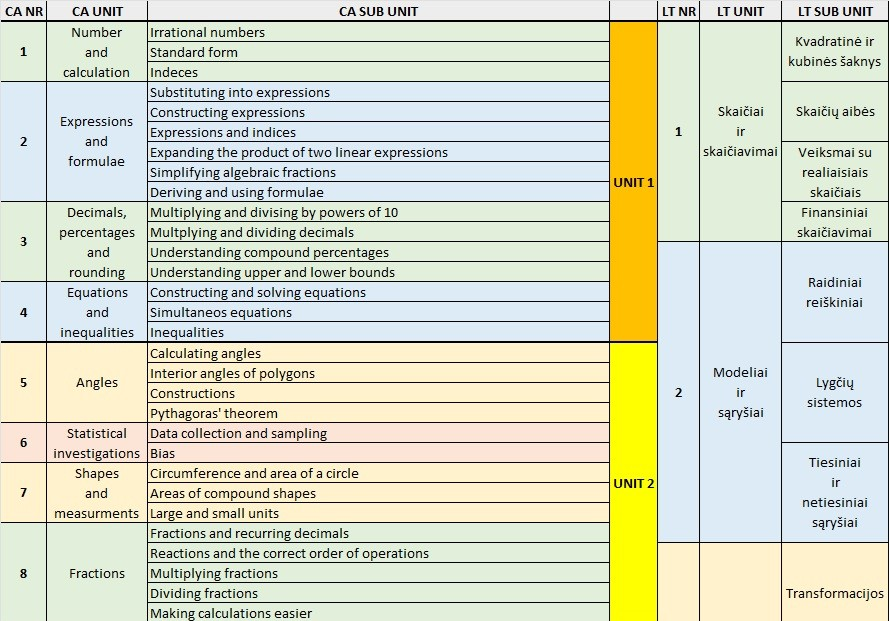
\includegraphics[scale=0.3]{mokymosi_turinys_up.jpg}
\end{minipage}
\hfill
\begin{minipage}{0.48\textwidth}
\centering
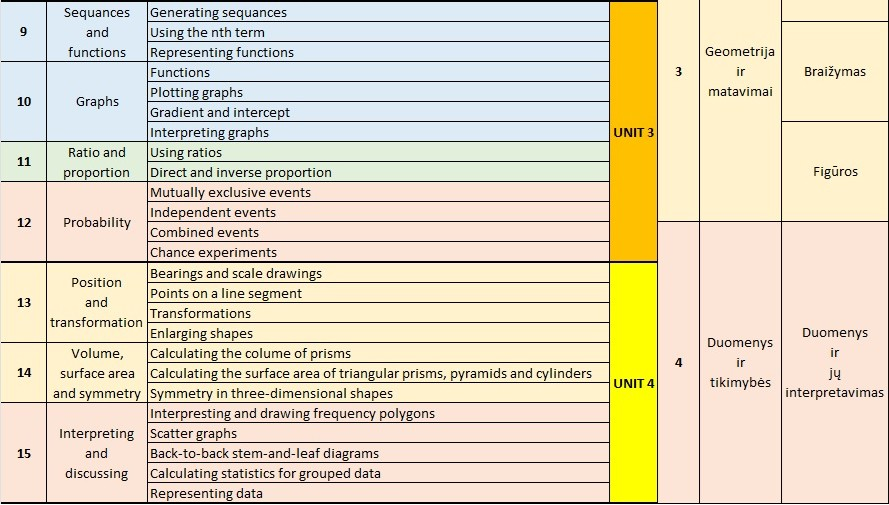
\includegraphics[scale=0.3]{mokymosi_turinys_bottom.jpg}
\end{minipage}
\end{frame}


\section{Diagnostiniai testai}